\section{LabVIEW als Programmiersprache}
	\label{sec:labview}
	
LabVIEW ist ein grafisches Programmiersystem von National Instruments. Das Akronym steht für "`Laboratory Virtual Instrumentation Engineering Workbench"'.
Die Programmierung erfolgt in der graphischen Programmiersprache "`G"'.  LabVIEW-Programme werden als Virtuelle Instrumente (VIs) bezeichnet. \cite{ni-tuto} %\cite{wiki-lv}
Sie bestehen aus drei Komponenten: 
\begin{description}
	\item[Frontpanel] - das User-Interface, über welches der Anwender mit dem VI interagiert
	\item[Blockdiagramm] - stellt den Programmcode des VIs dar
	\item[Anschluss] - dient zur Anbindung an weitere VIs, bestimmt Übergabe- und Rückgabe Werte
\end{description}

In LabVIEW liegt das Datenflussmodell der Ausführung von VIs  zugrunde. Ein Blockdiagrammknoten (Bsp. Addition) wird ausgeführt, sobald alle seine Eingänge belegt sind. 
Ist die Ausführung eines Knotens abgeschlossen, werden die Daten an die Ausgabeanschlüsse übergeben und die Ausgabedaten dann an den nächsten Knoten 
im Datenflussdiagramm weitergeleitet. \cite{labview-buch01}
Die unter LabVIEW erstellten Blockdiagramme werden von einem grafischen Compiler in optimierten Maschinencode übersetzt. 
Dadurch ist die Performance zur Laufzeit vergleichbar mit der anderer Hochsprachen wie C oder Pascal. 

Dieser Compiler ist der Schlüssel für die Produktivität von LabVIEW. Er abstrahiert Aufgaben wie die Speicherzuweisung und die Verwaltung von Threads. In der aktuellen LabVIEW Version 2010 wurde in den Compiler eine  "`Low-Level Virtual Machine"' (LLVM) aufgenommen. Die LLVM ist eine Open-Source-Compiler-Infrastruktur und soll die Codeausführung  beschleunigen. 
"`Die Architektur von LLVM basiert auf einer virtuellen Maschine (VM), die einen Prozessor virtualisiert. Die VM ist in der Lage, die intern generierte Sprache des Compilers während der Ausführung für den Prozessor des aktuellen Systems zu übersetzen."'\cite{lattner} Besonders hierbei ist, dass LLVM hocheffizient ist, was die Übersetzung auch in Echtzeit ermöglicht. \cite{llvm} \cite{ni-compiler}


Abbildung \ref{fig:demo01} zeigt eine Demonstration einer LabVIEW Applikation. Es wird aus den Eingängen A und B ein Ausgang C berechnet. Die Formel wird im Blockdiagramm abgebildet. Sie lautet:
\[ C = (\frac{A+B}{4})^{2} \]
Des Weiteren findet die Berechnung in einer While-Schleife statt. Die Abbruchbedingung ist die Betätigung der Stopp-Schaltfläche. 

	\begin{figure}%[h!]
	\centering
		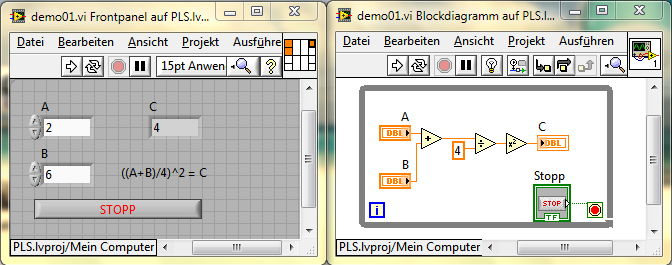
\includegraphics[width=0.7\textwidth]{Pics/demo01.png}
	\caption{VI Demonstration: Links Frontpanel, Rechts Blockdiagramm}
	\label{fig:demo01}
	\end{figure}

	%\subsection{Objektorientiertes Design}  %2-15
	\subsection{Entwurfsmuster - Design Patterns}
	\label{chap:entwurfsmuster}
Zur Entwicklung einer umfangreichen Applikation ist es unerlässlich mit Entwurfsmustern zu arbeiten. 
Sie helfen nicht nur dem Entwickler, den Überblick  zu behalten, sondern machen es auch für Außenstehende einfacher, den Code zu lesen und zu modifizieren.

LabVIEW bietet neun verschiedene Entwurfsmuster. Für welches man sich entscheidet, hängt von folgenden Kriterien ab:
\begin{itemize}
	\item Gibt es eine feste Reihenfolge / Sequenz von Befehlen?
	\item Muss das Programm mit einem User-Interface agieren?
	\item Ist die Datenverarbeitung intensiv? 
	\item Gibt es parallele Operationen?
\end{itemize}

Im Folgenden gehe ich auf einige Entwurfsmuster ein, die für die Problemstellung in Frage kommen. Das sind: der Zustandsautomat, das Master/Slave-Entwurfsmuster, 
der Ereignisbehandler für Benutzeroberfläche und das Erzeuger/Verbraucher-Entwurfsmuster. Später im Abschnitt \ref{chap:designpattern} werde ich auf die getroffene Wahl des Entwurfsmuster eingehen.

\subsubsection{Zustandsautomat}%4-6
Mit jedem Zustand wird ein bestimmter Blockdiagramm-Ausschnitt ausgeführt und ermittelt, zu welchem Zustand weitergesprungen wird. 
In einer While-Schleife wird eine Case-Struktur ausgeführt. 
%Die Case-Struktur erhält einen Initialisierungs-Zustand. In jedem Case der Case-Struktur wird auf eine anderen Case oder den eigenen Case weiter gesprungen bis die While-Schleife 
ihre Abbruchbedingung erreicht hat.
	
\subsubsection{Master/Slave-Entwurfsmuster}
Bei diesem Entwurfsmuster gibt es eine Master-Schleife und mindestens eine Slave-Schleife. Die Master Schleife wird immer ausgeführt. 
Sie benachrichtigt die Slave-Schleifen, einen bestimmten Code auszuführen. 
Die Slave-Schleifen werden vollständig ausgeführt und warten dann auf die nächste Benachrichtigung.

\subsubsection{Einfache Ereignisbehandlungsroutine für die Benutzeroberfläche}
Dieses Entwurfsmuster wird verwendet für die Verarbeitung von Ereignissen der Benutzeroberfläche. 
Die Vorlage eignet sich für Dialogfelder und andere Programmoberflächen. 
Des Weiteren kann man benutzerdefinierte Ereignisse erzeugen und ausführen, die wie Ereignisse der Benutzeroberfläche behandelt werden.

\subsubsection{Erzeuger/Verbraucher-Entwurfsmuster} %4-10 
Hier werden zwei separate While-Schleifen unabhängig voneinander ausgeführt: Die erste Schleife erzeugt Daten, während die zweite Schleife die Daten verarbeitet. 
Obwohl sie parallel ausgeführt werden, werden zwischen den Schleifen über Queues Daten ausgetauscht.
Diese Vorlage bietet die Möglichkeit, bei Benutzereingriffen asynchron Code auszuführen, ohne die Reaktionszeit der Benutzeroberfläche zu beeinträchtigen. 
So kann man durch die parallele Ausführung der Schleifen Leistungssteigerung des Programms erzielen. 

		
		%\paragraph{Event Handling}
		%\paragraph{Error Handling} %4-47
		
\section{Programmentwurf}
% cbcb besser: Programmentwurf
		%\subsection{Programmablaufplan} %2-18
\subsection{Datenabstraktion}
Um in LabVIEW auf Objekten zu arbeiten, gibt es Module. Das sind VIs die als Methoden agieren. Sie haben Eingänge und Rückgabewerte.
\subsubsection{Objekte}
Folgende Objekte werden in der Party-Licht-Steuerung unterschieden:
\begin{description}
\item[Lichtkanal]Eine Lampe mit einer Farbe, Intensität und Nummer.
\item[Lichterset]Ein 2D-Array aus Lampen mit einer Warte-, Überblendungs- und Nachlaufzeit sowie einem Namen.
\item[Lichterset Queue] Eine Liste aller nacheinander ablaufenden Lichtersets.

\item[Verbraucher-Queue]Die Warteschlange für die Verbraucherschleife - sie enthält Befehle der Erzeugerschleife für die Verbraucherschleife. 

%Das Objekt besteht aus einem Cluster mit: ein "`Kommando"' vom Typ "`Enum"' und einem "`Daten"' vom Typ Variant.

%Der Datentyp "`Variant"' ist ein allgemeiner Container für alle anderen Datentypen in LabVIEW. Sind Daten in ein Variantwert konvertiert, werden die Daten und der ursprüngliche Datentyp gespeichert. So kann LabVIEW die Variantdaten zu einen anderen Zeitpunkt wieder fehlerfrei in den ursprünglichen Datentyp umwandeln. \ref{LabViewHilfe}

\item[Display-Queue]Die Warteschlange für die Displayschleife - über diese kommuniziert die Verbraucherschleife mit der Displayschleife. 
%???ihr???.
% cbcb: Wer ist "ihr"?
%Sie enthält das selbe Cluster wie die Verbraucher-Queue.

\end{description}


\subsubsection{Module}
Dieser Abschnitt beschreibt die Module und nennt ihre Funktionen:
\begin{description}
\item[Lichterset-Modul] Das Lichterset-Modul initialisiert das Lichterset-Array und führt folgende Anweisungen darauf aus:
% cbcb: anweisungen solltest du kursiv schreiben und genau (addLichterset getLichterset, setLichterset)
	\begin{itemize}
	\item \textit{AddLichterset}, \textit{GetLichterset} und \textit{SetLichterset}
	\item \textit{getAnzahlLichtersets}
	\item \textit{getLeeresLichterset}
	\end{itemize}
%Ist eine FGV. Das Lichterset-Modul initalisiert ein 1D-Array aus Lichterset Objekten(Lichterset Queue) und führt die Anweisungen Add Get und Set sowie getAnzahl und getLeeresLichterset darauf aus.

\item[Display-Modul] Dieses Modul sorgt für die Aktualisierungen auf dem Front Panel.
	\begin{itemize}
	\item Initialisierung und Update des Front Panels
	\item Auswahl des Lichtersets aus der Lichterset-Queue
	\item De-/Aktivieren von Schaltflächen
	\item Update der Lichterset-Queue
	\end{itemize}

\item[Timing Modul] Das Modul sorgt für die Berechnung der verschiedenen Zeiten:
	\begin{itemize}
	\item Wartezeit
	\item Überblendungszeit
	\item Nachlaufzeit
	\end{itemize}
\item[Fehler Modul] Das Modul führt die Fehlerbehandlung durch.
	\begin{itemize}
	\item Fehler ausgeben
	\item Fehler behandeln
	\end{itemize}

\item[Datei Modul] Das Modul sorgt für die Datei- Ein- und Ausgabe.
	\begin{itemize}
	\item Speicher Lichtersets
	\item Lade Lichtersets
	\end{itemize}

\end{description}

Auf die Implementierung der Module wird im Kapitel \ref{chap:impl} eingegangen.

\subsection{Ablaufdiagramm }
Mit Ablaufdiagrammen wird der Programmfluss illustriert. Das Programm wird in handhabbare Funktionen und Verzweigungen gegliedert und dargestellt.
% Mit deren Hilfe kann man eine Aufgabe in handhabbare Funktionen teilen. 
Abbildung \ref{fig:plan01} zeigt das Ablaufdiagramm für die Abspiel-Funktion in der Party-Licht-Steuerung. 
Ein Knoten repräsentiert einen Zustand.
	\begin{figure}[!ht]
	\centering
		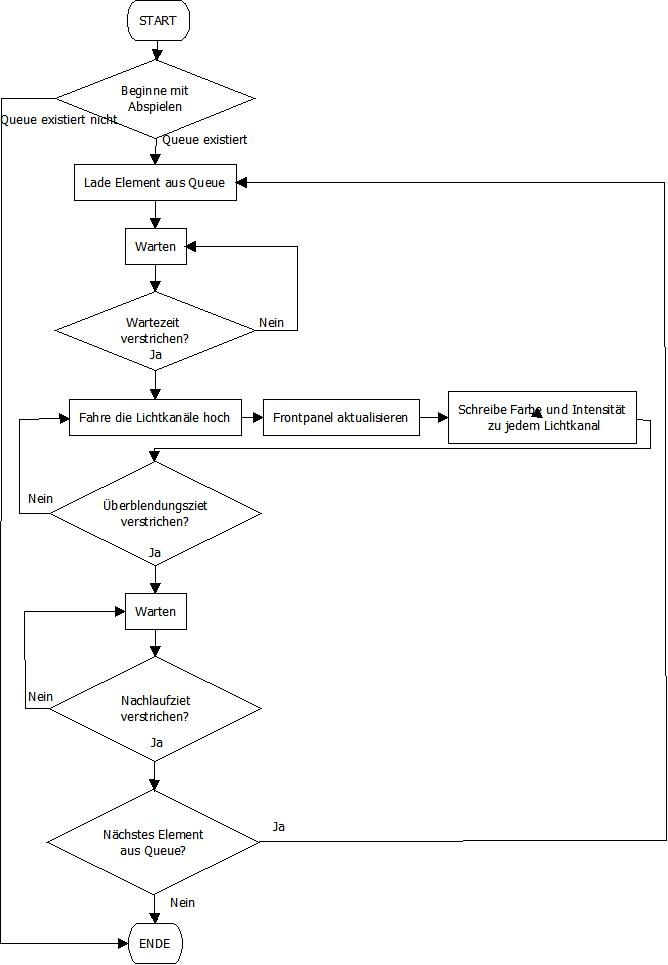
\includegraphics[height=0.9\textheight]{Pics/play-flowchart.jpeg}
	\caption{Ablaufdiagramm für die Abspiel-Funktion}
	\label{fig:plan01}
	\end{figure}	
		
\subsection{Datenflussdiagramm}
Datenflussdiagramme haben die Aufgabe, zu zeigen, welchen Weg die Daten durch eine Applikation nehmen. Abbildung \ref{fig:plan02} zeigt das Datenflussdiagramm für die Abspiel-Funktion
in der Party-Licht-Steuerung. Die Knoten (Kreise) repräsentieren die Prozesse. 
Eine externe Entität ist das Licht-Kontroll-System. Die Pfeile zeigen die Richtung des Datenflusses an.
	\begin{figure}[!ht]
	\centering
		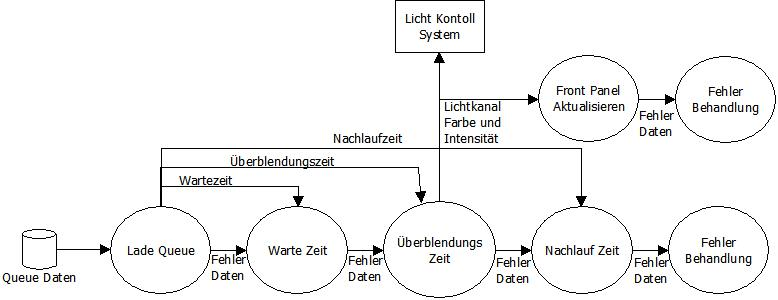
\includegraphics[width=\textwidth]{Pics/play-dataflow.jpeg}
	\caption{Datenflussdiagramm für die Abspiel-Funktion}
	\label{fig:plan02}
	\end{figure}	

	
%\section{User Interface}

\section{Implementierung}
\label{chap:impl}
		\subsection{Auswahl des Design Patterns} %6-3
		\label{chap:designpattern} %4-18
Bei der Wahl des Entwurfsmusters habe ich mich für das Erzeuger/Verbraucher - Entwurfsmuster (siehe Abschnitt \ref{chap:entwurfsmuster}) entschieden. 
Bei diesem Pattern kann man die Ereignisbehandlung vom User-Interface und dem auszuführenden Code gut trennen. 
Des Weiteren ist es möglich, die verschiedenen Schleifen parallel auszuführen.
Durch Hinzufügen weiterer Schleifen bleibt das Programm gut skalierbar. 
Ein anderer Grund für die Verwendung dieses Design Patterns ist die interne Kommunikation über Queues, das erleichtert das Steuern des User-Interfaces.

Das Entwurfsmuster wird wie folgt abgewandelt implementiert.  Die Erzeugerschleife reagiert auf Events vom User-Interface. 
Hauptbestandteile des User-Interfaces  sind die drei Schaltflächen: Abspielen, Aufnehmen und Stoppen sowie die Menüauswahl: Speichern, Laden und Beenden.

Über eine Verbraucher-Queue tauscht die Erzeugerschleife Kommandos und Daten mit der Verbraucherschleife aus. Hier sind folgende Kommandos implementiert:
\begin{itemize}
\item initialisieren
\item aufnehmen
\item abspielen
\item stoppen
\item laden
\item speichern 
\item beenden
\end{itemize}
Daten, welche die Erzeuger- an die Verbraucherschleife sendet, sind die Daten der Lampen-Sets die beim Aufnehmen, Speichern oder Laden entstehen. 
In der Verbraucherschleife werden alle Berechnungen durchgeführt. Die Verbraucherschleife kommuniziert über eine Display-Queue mit der Displayschleife.
Die Displayschleife hat die Aufgabe, Änderungen am User-Interface durchzuführen. Diese können sein:
\begin{itemize}
\item Initialisierung des Front Panels
\item Update der Lichtkanäle
\item Auswahl eines Lichtsets
\item Aktivieren und Deaktivieren von Schaltflächen
\item Update der Set-Ablaufliste
\item Stopp
\end{itemize}

Abbildung \ref{fig:schleifen} zeigt die Struktur aus dem Blockdiagramm. 
Die Funktionen der Applikation sind in drei separate Schleifen aufgeteilt. Der Vorteil dieser Architektur ist, 
dass die drei Schleifen parallel ausgeführt werden können. 
Des Weiteren ist diese Art der Architektur wartungsfreundlich und gut skalierbar. 

%Auf die Implementierung der einzelnen Funktionen wird in den folgenden Abschnitten eingegangen.

	\begin{figure}%[!ht]
	\centering
		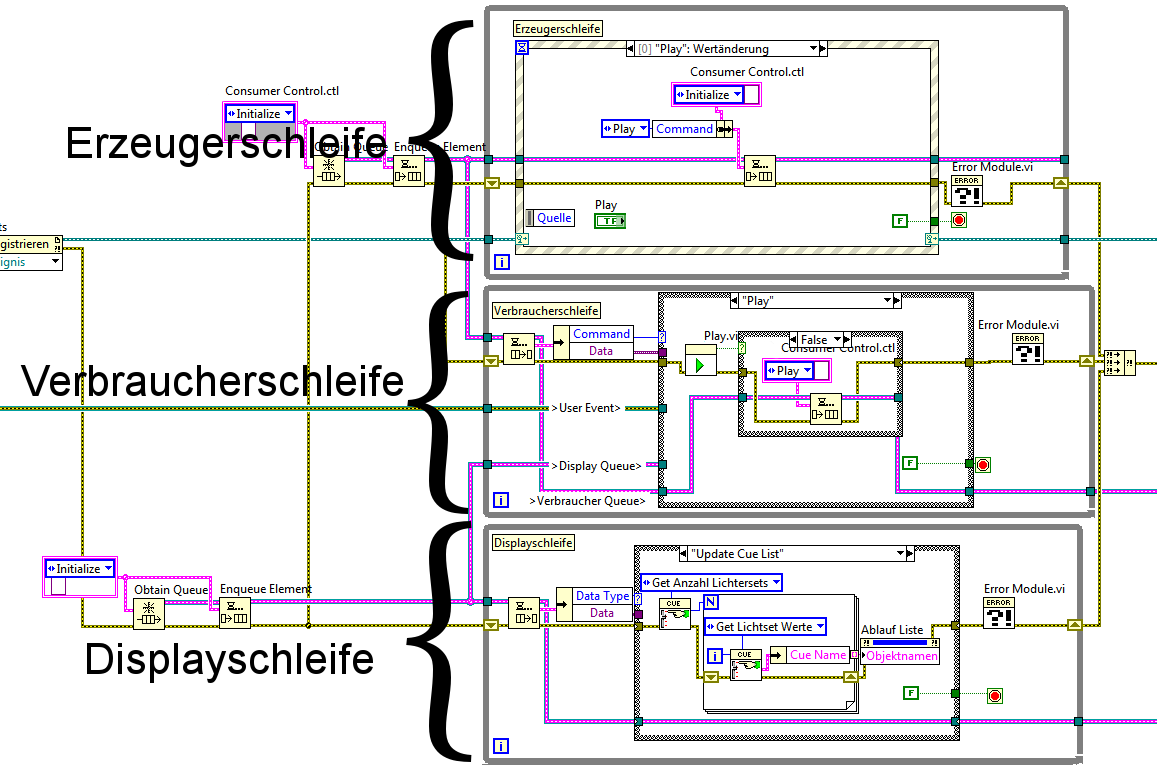
\includegraphics[width=\textwidth]{Pics/ueberblick004.png}
	\caption{Design Struktur für das Blockdiagramm}
	\label{fig:schleifen}
	\end{figure}
 		

		
		
		%\subsection{Timing}
		%\subsection{Auswahl der Datentypen}

\subsection{Init und Shutdown Funktion}	%E 7-1
Die Initialisierungsfunktion wird beim Start der Anwendung ausgeführt. Die setzt alle Module in einen definierten, sicheren Zustand und "säubert" das User-Interface. 
Abbildung \ref{fig:a1} im Anhang zeigt das Blockdiagramm vom \textit{"`init.vi"'}.

Wenn der Benutzer im Menü auf Datei$\rightarrow$Beenden klickt, wird die Anwendung sicher heruntergefahren, dass heißt, es werden alle Speicher-Referenzen freigegeben. 
Abbildung \ref{fig:a2} im Anhang zeigt das Blockdiagramm vom \textit{"`shutdown.vi"'}.

\subsection{User Interface}
Die Displayschleife sorgt für Updates auf dem User Interface.  Abbildung \ref{fig:disp} zeigt diese mit dem Stopp Case. Zu Beginn wird ein Element aus der Display Queue genommen
und dann nach Typ und Daten aufgeschlüsselt. 
Anhand des Datentyps, das  die Displayschleife von der Verbraucherschleife erhält, wird der entsprechende Case aufgerufen. Beim Kommando Stopp wird die While-Schleife beendet. 
Sollte ein Fehler in einem Case aufgetreten sein, wird dieser vom \textit{"`Error Module.vi"'} behandelt. Dazu mehr im Abschnitt \ref{chap:fehler} Fehlerbehandlung. 
Im Folgenden werden die einzelnen Cases in der Displayschleife erläutert.

	\begin{figure}[h!]
	\centering
		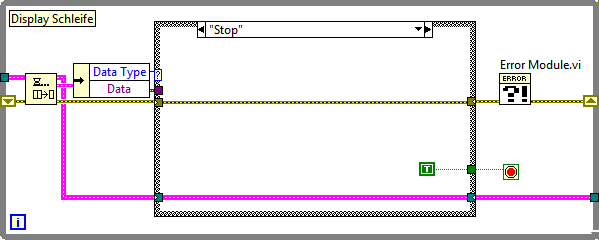
\includegraphics[width=\textwidth]{Pics/front-stop.png}
	\caption{Displayschleife}
	\label{fig:disp}
	\end{figure}

%Sie hat hat eine Case-Struktur mit den folgenden Funktionen.

\subsubsection{Initialisierung des Front Panels}
Dieser Case erstellt ein 2D-Array von Lichtkanälen und stellt es auf dem Front Panel dar. Jeder Kanal bekommt eine Nummer. Die Farbe wird auf schwarz und die Intensität auf 0 gesetzt. 

Der entsprechende Ausschnitt aus dem Programmcode ist im Anhang in Abbildung \ref{fig:a3} dargestellt.

\subsubsection{Auswahl eines Lichtsets aus der Lichterset Queue}
In diesem Case wird eine Spalte in der Ablaufkontrolle hervorgehoben, entweder wenn der User darauf klickt oder wenn die Applikation beim Abspielen über die Queue von Lichtersets iteriert. 

Der entsprechende Ausschnitt aus dem Programmcode ist im Anhang in Abbildung \ref{fig:a4} dargestellt.
 
\subsubsection{Aktivieren und Deaktivieren von Schaltflächen}
Wenn eine Lichterset Queue abgespielt wird, schaltet dieser Case die Schaltfläche Aufnehmen und die Ablaufkontrollliste inaktiv. 
Das verhindert, dass der Nutzer während eines Abspielvorgangs ein neues Lichterset anlegt und die Ablaufkontrollliste "durcheinander bringt".

Der entsprechende Ausschnitt aus dem Programmcode ist im Anhang in Abbildung \ref{fig:a5} gezeigt.

\subsubsection{Update der Set-Ablaufliste}
Dieser Case aktualisiert die Liste in der Ablaufkontrolle wenn ein neues Lichterset aufgenommen wurde.

Der entsprechende Ausschnitt aus dem Programmcode ist im Anhang in Abbildung \ref{fig:a6} gezeigt.

\subsubsection{Update der Lichtkanäle}
Dieser Case aktualisiert das 2D-Array aus Lichtkanälen. Es wird immer dann aufgerufen, wenn sich Lichtkanal-Daten ändern. 
Das ist der Fall, wenn eine Lichterset Queue abgespielt wird und sich die Farbe und Intensität der Kanäle ändert oder der Nutzer auf ein Element in der Ablaufkontolle klickt
um  Informationen zum ausgewählten Lichterset anzuzeigen.

Der entsprechende Ausschnitt aus dem Programmcode ist im Anhang in Abbildung \ref{fig:a7} dargestellt.


\subsection{Aufnahme-Funktion}	
Klickt der Anwender auf die Aufnahme Schaltfläche, öffnet sich eine Dialogbox in welcher der Nutzer nach Parametern für das zu erstellende Lichterset gefragt wird. 
Die einzugebenden Werte sind:
\begin{itemize}
\item Setname
\item Wartezeit
\item Überblendungszeit
\item Nachlaufzeit
\item Einstellungen für die einzelnen Lichtkanäle
\end{itemize}

Nach Bestätigung über die OK-Schaltfläche werden die gesammelten Daten in die Queue geschrieben und das User-Interface aktualisiert. 

Die Abbildung \ref{fig:rec} zeigt die Erzeuger-(oben) und Verbraucherschleife(unten). In der Erzeugerschleife wird die Dialogbox geöffnet. 
Sie gibt ein Objekt mit den gesammelten Daten zurück. 
Wurde der Dialog nicht abgebrochen, werden die Daten zusammen mit dem Kommando "`record"' in die Verbraucher Queue gesteckt. 
Die Verbraucherschleife nimmt  das Objekt aus der Queue und hängt das neue Objekt an die Lichterset-Liste an. 
Dann gibt sie das Kommando zum Aktualisieren des User-Interfaces an die Displayschleife.

	\begin{figure}[!ht]
	\centering
		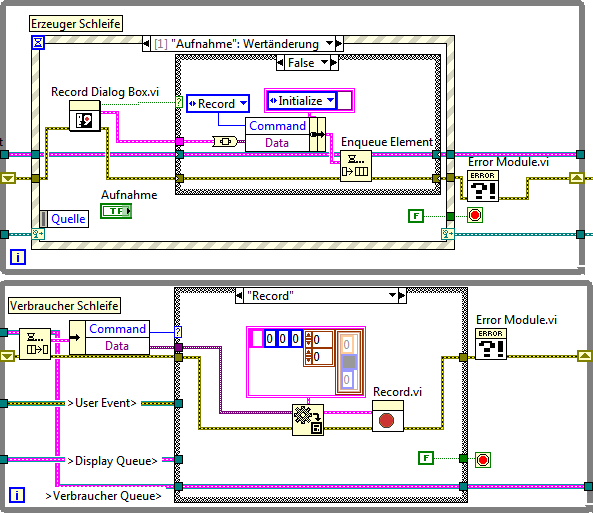
\includegraphics[width=\textwidth]{Pics/record.png}
	\caption{Aufnahme-Funktion}
	\label{fig:rec}
	\end{figure}
	
	
\subsection{Timing}
\label{chap:timing}
Zur akkuraten Berechnung der Warte-, Überblendungs- und Nachlaufzeit beim Abspielen der Lichtersets dient das Timing VI. 
Dieses VI arbeitet als funktionale globale Variable (FGV).

\subsubsection{Funktional globale Variable}
In funktionalen globalen Variablen  können in nicht initialisierten Schieberegistern von While- oder For-Schleifen Daten gehalten werden. 
Die Daten bleiben erhalten, solange sich das zugehörige VI im Speicher befindet. Die jeweilige Schleife in einer FGV wird bei einem Aufruf nur einmal durchlaufen. 
Liegen die Daten am Ende der Schleife (rechts) im Schieberegister an, stehen diese beim nächsten Aufruf wieder am Anfang (links) an. 
Das hat den Vorteil, dass Daten nicht immer bei jedem VI Aufruf mitgeführt werden müssen. 
Die Daten werden einmal beim Initialisieren mitgegeben und halten sich dann im Speicher. \cite{LabViewHilfe}

Die Timing FGV hat zwei Kommandos: starten(initialisieren) und checken. 
Die Auswahl wird über eine Switch-Case-Anweisung getroffen. Soll eine Zeit gemessen werden, 
wird zu Beginn der Messung das Timing VI mit der Ziel-Zeit und dem Kommando Start aufgerufen. 
Hier wird die aktuelle Systemzeit in Sekunden ermittelt (Startzeit) und ins Schieberegister geschrieben. 
In der Applikation wird in einer Schleife im Anschluss mit dem Kommando check abgefragt, ob die Zeit abgelaufen ist. 
Ist das der Fall, gibt die FGV am Ausgang "`Verstrichen"' True zurück, sonst False. 
Abbildung \ref{fig:timing} zeigt die FGV mit ihren beiden Cases. 

	\begin{figure}[h!]
	\centering
		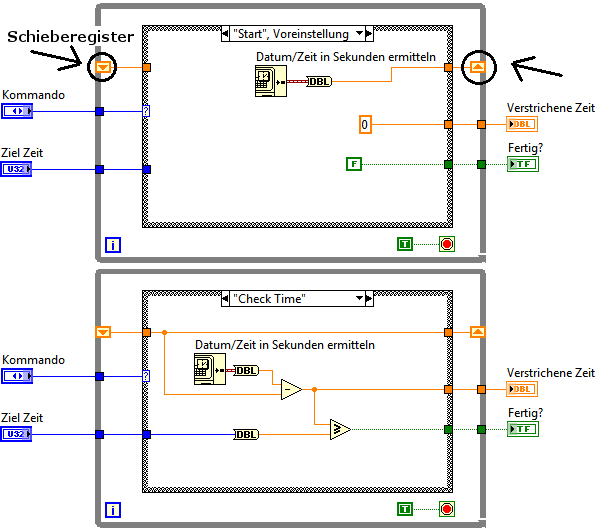
\includegraphics[width=\textwidth]{Pics/timing.png}
	\caption{FGV Timing VI}
	\label{fig:timing}
	\end{figure}


\subsection{Abspiel-Funktion}
Die Abspiel-Funktion wird als Zustandsautomat implementiert. Das Flussdiagramm aus Abbildung \ref{fig:plan01} zeigt die einzelnen Zustände. 

Empfängt die Verbraucherschleife das Kommando zum Abspielen, öffnet sie das \textit{"`record.vi"'}. Das VI durchläuft einen Zustand. 
Gibt es zurück, dass der Zustandsautomat noch nicht bis zum Ende durchgelaufen ist, steckt die Verbraucherschleife erneut das Kommando play in die Verbraucher Queue. 
Daraus resultiert eine Schleife, in der bei jeder Iteration ein Zustand durchlaufen wird, solange bis der Zustandsautomat am Ende ist.
Zur Berechnung, ob die verschieden Zeiten abgelaufen sind, wird das  \textit{"`timing.vi"'} aufgerufen. 
Im Anhang in Abbildung \ref{fig:a9} findet sich der Code für den Zustand Überblenden.

\subsection{Stopp-Funktion}
Will der Bediener den Abspiel-Vorgang abbrechen, klickt er auf die Stopp Schaltfläche. Jetzt wird der Zustandsautomat der Abspiel-Funktion unterbrochen. 
Das geschieht, indem die Verbraucher Queue geleert und der Zustandsautomat zurückgesetzt wird. 
So wird garantiert, dass keine Nachrichten mehr in der Verbraucher-Queue sind und der Zustandsautomat beim nächsten Anlauf wieder am Anfang startet. 
Der Code ist im Anhang in Abbildung \ref{fig:a10} gezeigt.
		
		
\subsection{Speichern und Lade Funktion}
Die Funktionalität zum Speichern und Laden in eine Datei ist für ein LJ unerlässlich. 
So kann der LJ während einer Probe alle Einstellungen setzen und diese in einer Datei speichern. 
Zum Zeitpunkt des Events muss die Datei nur noch geladen werden. 

Zum Speichern oder Laden klickt der LJ in die Menüleiste unter Datei auf Speichern bzw. Laden. Die Applikation (Erzeugerschleife) öffnet einen File-Dialog 
und prüft, ob die ausgewählte Datei existiert. 
Dann schickt sie das entsprechende Kommando (load oder save) zusammen mit dem Dateipfad an die Verbraucherschleife.

\subsubsection{In Datei speichern}
In der Verbraucherschleife wird über eine For-Schleife ein 1D-Array aus Lichtersets erstellt. Dieses wird an das \textit{"`File-Modul.vi"'} übergeben. 
Hier wird das 1D-Array in die angegebene Datei geschrieben. 
Hierfür werden die vorgefertigten LabView VIs genutzt: Öffnen, Schreiben und Schließen einer Datei. Der Code ist im Anhang in Abbildung \ref{fig:a11} dargestellt.

\subsubsection{Aus Datei laden}
Um aus einer Datei Elemente lesen zu können, muss man der Lese-Funktion den Lichterset Datentyp mitgeben. 
Zurück bekommt man ein 1D-Array aus Lichtersets. Die Elemente dieses Arrays werden dann in die Lichterset Queue geschrieben. 
Der Code ist im Anhang in Abbildung \ref{fig:a12} dargestellt.


\subsection{Fehlerbehandlung}
\label{chap:fehler}
Zur Fehlerbehandlung gehört das sichere Herunterfahren der Applikation wenn ein Fehler auftritt. Um die Erzeugerschleife zu beenden,
muss ein User-Event erzeugt werden. Die Verbraucherschleife wird beendet indem das Kommando Exit in die Verbraucher Queue geschrieben wird. 
Zum Beenden der Displayschleife wird das Kommando Stopp an die Display Queue gesendet. 
Empfängt eine Schleife  ein Stopp-Kommando bzw. Event wird die Abbruchbedingung auf true gesetzt. 
Sind alle drei Schleifen beendet, wird in der letzten Sequenz der Applikation die Verbraucher- und Display-Queue freigegeben, 
die Ereignisregistrierung aufgehoben, die Benutzerereignisse gelöscht, der aufgetretene Fehler ausgegeben und die LabVIEW Anwendung beendet.

Der Code, der im Fall eines oder mehrere Fehler ausgeführt wird, ist im Anhang in Abbildung \ref{fig:a13} zu finden.

\section{Funktionstest}

Bei einem funktionsorientierten Test wird ein Modul auf seine Spezifikationen geprüft. Exemplarisch wird hier das Timing Modul einem Black-Box-Funktionstest unterzogen. Das heißt, das die genaue Beschaffenheit des Moduls nicht betrachtet wird. Nur nach außen sichtbares Verhalten fließt in den Test ein.

Die Spezifikation kann dem Abschnitt \ref{chap:timing} entommen werden.  Das Modul verfügt über folgende Eingänge:

\begin{description}
\item[Kommando] Gibt an, was das Modul tun soll. Der Datentyp ist eine Typdefinition mit einem Enum aus Strings(start und check).
\item[Zielzeit] Gibt die Zeit in Sekunden deren Ablauf geprüft werden soll. Der Datentyp ist ein 32 Bit langes vorzeichenloses Long. Gültig sind Werte im Bereich von 0 bis 4.294.967.295.
\item[Fehler] Enthält Fehler Informationen von vorangegangenen VIs. 
\end{description}
Die Ausgänge des Moduls sind:

\begin{description}
\item[Verstrichene Zeit] Gibt die Zeit an, die seit dem Start verstrichen ist. Der Datentyp ist ein 64 Bit Double.
\item[Fertig] Ein Boolean der true zurück gibt wenn die Zielzeit abgelaufen ist und false wenn die Zeit noch läuft.
\item[Fehler] Gibt Fehler aus, die im VI oder durch vorangegangene VIs entstanden sind.
\end{description}

Folgende Testfälle werden auf dem Modul ausgeführt. Als Testwerkzeug dient das Frontpanel des VIs und eine Stoppuhr.

\begin{figure}[!ht]
\centering

\begin{tabular}{p{2cm}|p{5.2cm}|p{5.2cm}|p{2.5cm}}
	 Zeit [s] & Eingabe Parameter & Erwartete Ausgabe & Test Resultat \\ 
\hline 
	0 & 
	Kommando: start\newline Zielzeit: 5\newline kein Fehler & 
	Fertig: false\newline Verstrichene Zeit: 0\newline kein Fehler &
	erfolgreich \\ 
\hline 
	3 & 
	Kommando: check\newline Zielzeit: 5\newline kein Fehler & 
	Fertig: false\newline Verstrichene Zeit: 3\newline kein Fehler & 
	erfolgreich \\ 
\hline 
	6 & 
	Kommando: check\newline kein Fehler & 
	Fertig: true\newline Verstrichene Zeit: 6\newline kein Fehler & 
	erfolgreich \\ 
\hline 
	10 & 
	Kommando: start\newline  Zielzeit: -3\newline kein Fehler & 
	Fertig: false\newline Verstrichene Zeit = 0\newline Fehler: "negative Startzeit"' & 
	erfolgreich \\ 
\hline 
	15 & 
	Kommando: start\newline Zielzeit: 5\newline Fehler:"`Queue Daten Error"' & 
	Fertig: false\newline Verstrichene Zeit: 0\newline Fehler: "`Queue Daten Error"' & 
	erfolgreich \\
\hline  
	20 & 
	Kommando: check\newline Zielzeit: 5\newline Fehler:"`Queue Daten Error"' & 
	Fertig: false\newline Verstrichene Zeit: 0\newline Fehler: "`Queue Daten Error"' & 
	erfolgreich \\ 
\end{tabular} 

\caption{Testfälle Timing Modul}
\label{fig:test-time}
\end{figure}
Alle Testfälle konnten erfolgreich abgeschlossen werden. Somit ist der Funktionstest für das Timing Modul bestanden.



\section{Stress- und Ladetest}		
Bevor die Anwendung freigegeben wird, ist es notwendig, die Leistung und Handhabbarkeit der Applikation zu testen. 

Für den Test der Party-Licht-Steuerung wird ein VI geschrieben das 10.000 Lichtersets mit zufälligen Parametern für die Warte-, Überblendungs- und Nachlaufzeit sowie Lichtfarbe und -intensität
in eine Datei schreibt. 

Als Testwerkzeug dient der Windows Task-Manager. Er läuft mit während die Testdatei in die Anwendung geladen und abgespielt wird.
Mit Hilfe des Windows Task-Managers kann überprüft werden, ob während der Laufzeit ein Leistungs- oder Speicherfehler auftritt. 

Die Anwendung wurde auf einem Notebook mit einem Intel Core2 Duo Prozessor (2,17GHz) und 2 GB Hauptspeicher ausgeführt. 

Abbildung \ref{fig:test} zeigt den Verlauf der Prozessor- und Arbeitsspeicher Auslastung während des Tests. 
Das erste rot umrahmte Viereck (von links nach rechts) zeigt den Ladevorgang der Applikation. Es werden circa 40 MB in den Arbeitsspeicher geladen. 
Das zweite Viereck umrahmt das Laden der Testdatei (2,7 MB) hierfür werden im Arbeitsspeicher ungefähr 102 MB reserviert. 
Damit beansprucht die gesamte Applikation 141 MB des Hauptspeichers. 
Das letzte Viereck zeigt  den Abspielvorgang bis zum 140. Lichterset. 
Nach ungefähr 4 Stunden sind alle 10.000 Sets durchgelaufen danach konnte die Anwendung ohne Fehler beendet werden.
Der zuvor reservierte Speicher wurde wieder freigegeben. 
Während des Abspielvorgangs war der Prozessor im Mittel mit 14\% ausgelastet.

% Der Test zeigt die folgenden wesentlichen Ergebnisse:, das kein Speicherüberlauf auftrat,
% kein Speicher unnötig allokiert wurde und der Prozessor mit der Anwendung nicht überlastet war.

\begin{itemize}
\item Die Anwendung verursacht keinen Speicherüberlauf.
\item Es wird kein Speicher unnötig allokiert.
\item Der Prozessor ist mit der Anwendung nicht überlastet.
\end{itemize}
 Somit gilt der Test als bestanden. 

	\begin{figure}%[]
	\centering
		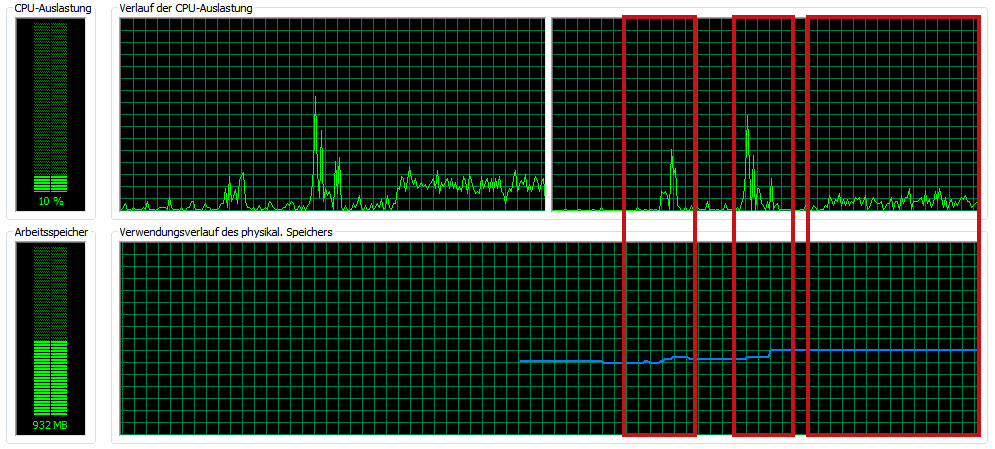
\includegraphics[width=\textwidth]{Pics/test04.png}
	\caption{Verlauf der Prozessor- und Arbeitsspeicher Auslastung}
	\label{fig:test}
	\end{figure}




\section{Einsatz der Anwendung}
LabVIEW bietet die Möglichkeit, über einen Dialog aus einem Projekt heraus eine ausführbare Windows- (.exe) oder MAC OS (.app) Anwendung wahlweise mit Installer zu erstellen. 
Eine ausführbare Windows-Anwendung und ein Installer mit der notwendigen Laufzeit-Umgebung finden sich auf der beigefügten CD. 
Für die Laufzeit-Umgebung gibt es eine kostenfreie Lizenz, sie kann beliebig oft vervielfältigt werden.

Die Mindestvoraussetzungen für die Windows-Laufzeitumgebung sind \cite{ni-min}: 
\begin{itemize}
\item Prozessor: Pentium III/Celeron 866 MHz oder gleichwertig
\item Hauptspeicher: 256 MB
\item Festplattenspeicher: 1 GB
\item Betriebssystem: XP
\end{itemize}
%http://www.ni.com/labview/requirements/d/

\subsection{Webservice}

% cbcb: Sehr dünn, was du  zu Webservicen schreibst
% Schau mal nochmal  in LabView nach, was für ein Interface/Protokoll benutzt/erstellt wird (SOA, Axis??, RPC??) und was den Client und was den Server-Teil bildet 
% und was, wo zu installieren ist und wie der Webservice angesprochen wird vom Client

Mit LabVIEW lässt sich ein Webservice erstellen, auf den der Anwender via Inter- oder Intranet mit einem Standard-Browser zugreifen kann. 
Rechenintensive Anwendungen können von einem Server  bearbeitet werden und müssen nicht die Rechnerressourcen des Clients beanspruchen. 
Mit einem Webservice lassen sich Prozesse von der Ferne aus überwachen. Anwendungen hierfür sind zum Beispiel die Produktionsüberwachung und Produktionssteuerung von Maschinen. Mitarbeiter müssen nicht von Maschinenterminal zu Maschinenterminal laufen sondern könnten zum Beispiel von einem Heimarbeitsplatz via Internet eine ganze Produktionsanlage überwachen.

VIs können von jedem HTTP-fähigen Web-Client aus unter Angabe einer URL  aufgerufen werden. 
Der Austausch von Daten kann dann mit herkömmlichen HTTP-Methoden wie POST erfolgen. 

Web-Clients tauschen Daten mit einer Webdienstapplikation aus, indem sie HTTP-Anfragen an definierte URLs senden. 
Der Webdienst akzeptiert die Anfrage und sendet Daten im XML-, HTML-, JSON- oder TXT-Format zurück an den Web-Client. 
Ein Web-Client kann beispielsweise eine Anfrage mit zwei Werten an einen Webdienst senden, der dann die Summe aus diesen Werten bildet und das Ergebnis an den Client sendet. \cite{LabViewHilfe}





\section{Abschließende Betrachtung}
Bei dem Projekt ist eine voll funktionsfähige LabVIEW Anwendung entstanden, somit konnte das Projekt erfolgreich abgeschlossen werden. 

\subsection{Fazit}
Ein wichtiger Vorteil in der graphischen Programmierung von LabVIEW ist die Einfachheit, parallele Abläufe zu programmieren. 
So reicht es aus, zwei Sub-VIs ohne Datenabhängigkeit nebeneinander zulegen. 
Man muss jedoch auf mögliche "`Race Conditions"'
	\footnote{Race Condition: Ein kritischer Wettlauf, auch Wettlaufsituation ist 	in der Programmierung eine Konstellation, in der das Ergebnis einer Operation vom zeitlichen Verhalten bestimmter Einzeloperationen abhängt.\cite{wiki-RC} } 
achten.



Hierfür stehen verschiedene Möglichkeiten zur Verfügung. 
Zum Beispiel Semaphore oder Warteschlangen. 
% cbcb: Semaphore und Wartescchlange musst du auch erklären

Die Umsetzung des Projekts über das Front Panel von LabVIEW hat gezeigt, dass es eine bequeme Möglichkeit bietet, schnell eine einfache und  gute Bedienoberflächen zu erstellen.

% Im Blockdiagramm ist durch die graphische Darstellung des Programmablaufs die Lesbarkeit deutlich einfacher
% cbcb einfacher als was? einfacher Deshalb besser:

Das Blockdiagramm ermöglicht durch die graphische Darstellung des Programmablaufs eine gute Lesbarkeit.
Anhand verschiedener Farben lassen sich die Datentypen und ihr Ursprung gut erkennen.

Ein weiterer Vorteil, den LabVIEW bietet, ist die Unterstützung von Kommunikationsprotokollen wie TCP/IP. 
Es ist somit möglich auch  entfernte Anwendungen zu steuern und zu nutzen.

Bei der Entwicklung von LabVIEW Programmen gibt es auch Nachteile.
So ist man an die originale LabVIEW-Entwicklungsumgebung von National Instruments gebunden. 
Für diese fallen Lizenze-Kosten an. Die "`NI Developer Suite Core"' für Windows kostet 5.800 Euro.
Hier gibt es auch kostenlose Versionen mit vermindertem Funktionsumfang für Studenten. \cite{ni-kost}
%http://ohm.ni.com/advisors/devsuite/pages/cds/newcustomer.xhtml

Auf einen weiteren Nachteil stößt man, wenn man LabVIEW-Programme verteilen will. Hat das Zielsystem keine Entwicklungsumgebung, ist es nötig, eine Laufzeitumgebung zu installieren.
Diese ist für die meisten Module kostenfrei.

% cbcb
%Änderungsfreundlichkeit:
Auch bei strukturierter Programmierung können kleine Änderungen im Programmfluss  aufwendige Neustrukturierungen nach sich ziehen. 
Ärgerlich ist es, beim Schaffen vom Raum im Blockdiagramm immer wieder Drähte und Symbole neu ordnen zu müssen.

Abschließend lässt sich sagen, das LabVIEW trotz der beschriebenen Nachteile eine adäquate Lösung bietet, Programme schnell und effizient zu entwickeln. %  gutes Aufwand/Nutzen Verhältnis


	
\subsection{Ausblick auf Erweiterungen}
Die umgesetzte Party-Licht-Steuerung bietet Möglichkeiten für Erweiterungen.

\subsubsection{Ansteuerung von Hardware}
Möchte man externe Lichtkanäle ansteuern, könnte man ein dritte Verbraucherschleife hinzufügen. 
Diese muss dann einen "`Data Acquisition-Task"' starten und die Ausgänge setzen. 
Als anzusteuernde Hardware empfiehlt sich das NI PCI-6723 Analogausgangsmodul. 
Es hat 32 Analogausgänge, damit könnte man  Farbe und Intensität von 16 Lampen steuern.\cite{ni-pci}

	\begin{figure}[h!]
	\centering
		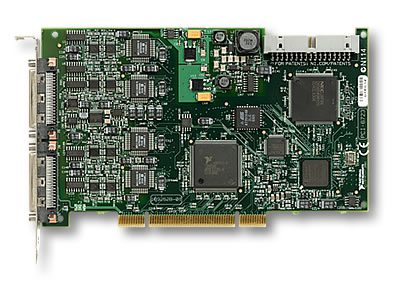
\includegraphics[width=0.5\textwidth]{Pics/pci6723.jpg}
	\caption{NI PCI-6723 mit 32 Analogausgänge \cite{ni-pci} }
	\label{fig:a7}
	\end{figure}

%http://sine.ni.com/nips/cds/view/p/lang/de/nid/12551



\subsubsection{Multilingualität}
Um die Applikation einer größeren Zahl an Anwendern zur Verfügung zu stellen, kann eine Mehrsprachigkeit implementiert werden. 
Dazu kann der Nutzer beim Start der Anwendung  nach seiner präferierten Sprache gefragt werden. Über eine Tabelle mit den zur Verfügung stehenden Sprachen kann
eine Auswahl für die Beschriftung der Front Panel Elemente getroffen werden.





